% =====================================================================
%  PHỤ LỤC D. MINH CHỨNG SẢN PHẨM ĐỀ TÀI
% =====================================================================
\chapter{Minh chứng sản phẩm đề tài}
\label{pl:d}

\section{Danh mục sản phẩm nộp kèm}

\begin{table}[H]
\centering
\caption{Danh mục sản phẩm nộp kèm hồ sơ nghiệm thu}
\small
\renewcommand{\arraystretch}{1.2}
\begin{tabularx}{\textwidth}{@{}c>{\raggedright\arraybackslash}p{4.6cm}>{\raggedright\arraybackslash}X@{}}
\toprule
\textbf{STT} & \textbf{Sản phẩm} & \textbf{Tệp / nội dung}\\
\midrule
1 & Chương trình máy tính & Thư mục mã nguồn \texttt{pfdet\_drone\_follow} (Phụ lục~B)\\
2 & Mô hình triển khai & \texttt{pfdet\_v17\_640\_coco\_hailo8l.hef} (INT8, Hailo-8L)\\
3 & Video bay thử & \texttt{video/video\_bay\_thu.mp4}: phần 1 phát hiện người trên video bay thử; phần 2 vòng bám người trên cùng chuyến bay\\
4 & Nhật ký vòng bám người & \texttt{video/replay\_log.csv}: trạng thái, mục tiêu khoá, sai số hướng, lệnh quay hướng của từng khung\\
5 & Báo cáo tổng kết & Tài liệu này\\
6 & Bài tóm tắt đề tài & \texttt{tomtat/tomtat.docx} (2 trang, 2 cột)\\
7 & Poster (mẫu BM07A) & \texttt{poster\_a3/poster\_a3.pdf} (A3 ngang, Phụ lục~E) và \texttt{poster\_a3/poster\_a1.pdf} (A1)\\
8 & Standee (mẫu BM07B) & \texttt{standee/standee.pdf} (0,6 $\times$ 1,6\,m)\\
9 & Bài trình bày trước hội đồng & \texttt{slides/slides.pdf}\\
\bottomrule
\end{tabularx}
\end{table}

\section{Hình ảnh sản phẩm}

\begin{figure}[H]
\centering
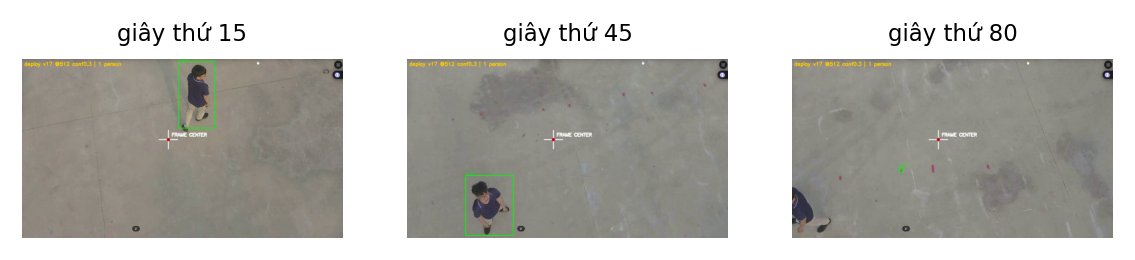
\includegraphics[width=\textwidth]{demo_khung.png}
\caption{Phần 1 của video bay thử: SteadyDet-N phát hiện người trên các khung hình của chuyến bay 21/07/2026}
\end{figure}

\begin{figure}[H]
\centering
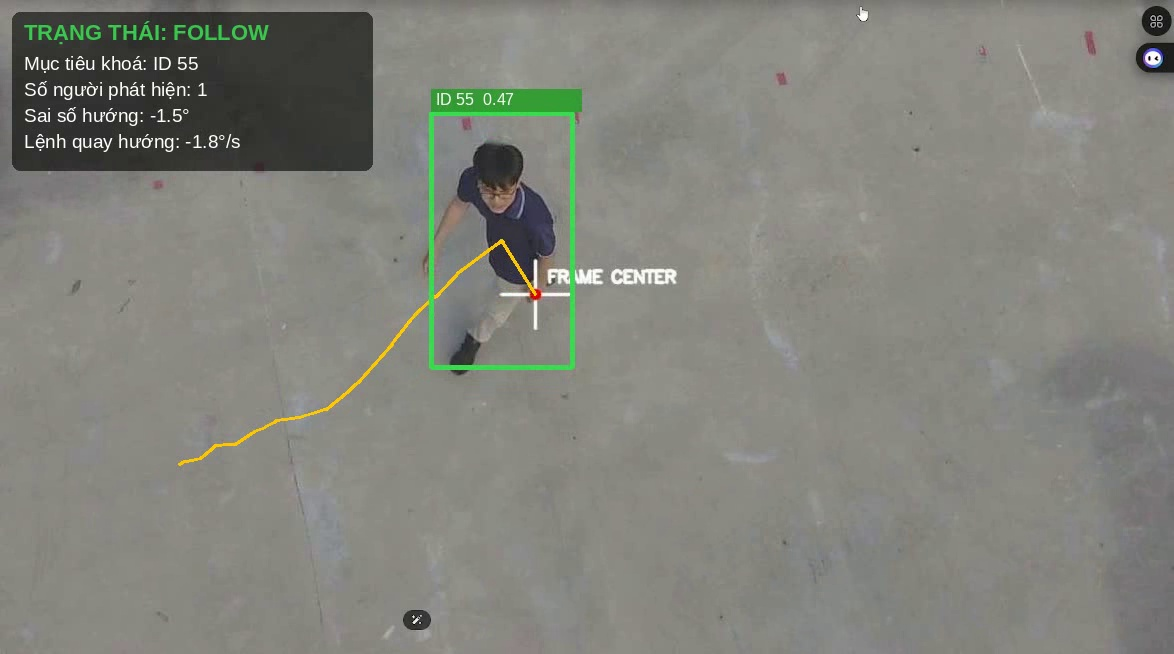
\includegraphics[width=0.8\textwidth]{vongbam_2.jpg}
\caption{Phần 2 của video bay thử: vòng bám người khoá mục tiêu, hiển thị trạng thái, sai số hướng và lệnh quay hướng}
\end{figure}
